% 2010 全国卷理科第 18 题：等腰梯形底面的四棱锥示意图。
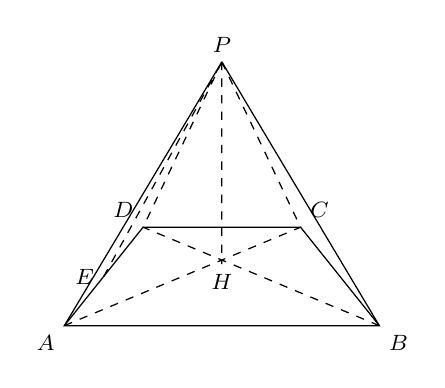
\begin{tikzpicture}[font=\footnotesize, line width=0.45pt]
  \coordinate (A) at (0,0);
  \coordinate (B) at (4.0,0);
  \coordinate (D) at (1.0,1.25);
  \coordinate (C) at (3.0,1.25);
  \coordinate (H) at (2.0,0.78);
  \coordinate (P) at (2.0,3.35);
  \coordinate (E) at (0.5,0.625);
  \draw (A)--(B)--(C)--(D)--cycle;
  \draw[dashed] (A)--(C) (B)--(D) (P)--(H) (P)--(D) (P)--(C) (E)--(P);
  \draw (P)--(A) (P)--(B);
  \node[below left] at (A) {$A$};
  \node[below right] at (B) {$B$};
  \node[above left] at (D) {$D$};
  \node[above right] at (C) {$C$};
  \node[above] at (P) {$P$};
  \node[below] at (H) {$H$};
  \node[left] at (E) {$E$};
\end{tikzpicture}
